\section{Dynamic Scheduling}
\label{sec:scheduling}
Once static compilation produces an executable generalized PCG for a \peft model, \sys must determine an execution schedule capable of concurrently handling both finetuning and inference requests.
%
This is particularly challenging due to the distinct characteristics of these two workloads. 
%
First, inference requests arrive in an online and highly dynamic manner, requiring the system to rapidly adapt GPU resource allocation to maintain low-latency responses. In constrast, finetuning involves both a forward pass---similar to inference---and a backward pass to update model parameters. 
Additionally, auto-regressive inference for generative LLMs proceeds in a token-by-token fashion, while finetuning is typically performed at the sequence level to maximize throughput.
To address these challenges, \sys introduces a novel \textit{token-level finetuning} mechanism along with a \textit{hybrid token scheduler}.

\begin{figure}[t]
    \centering
    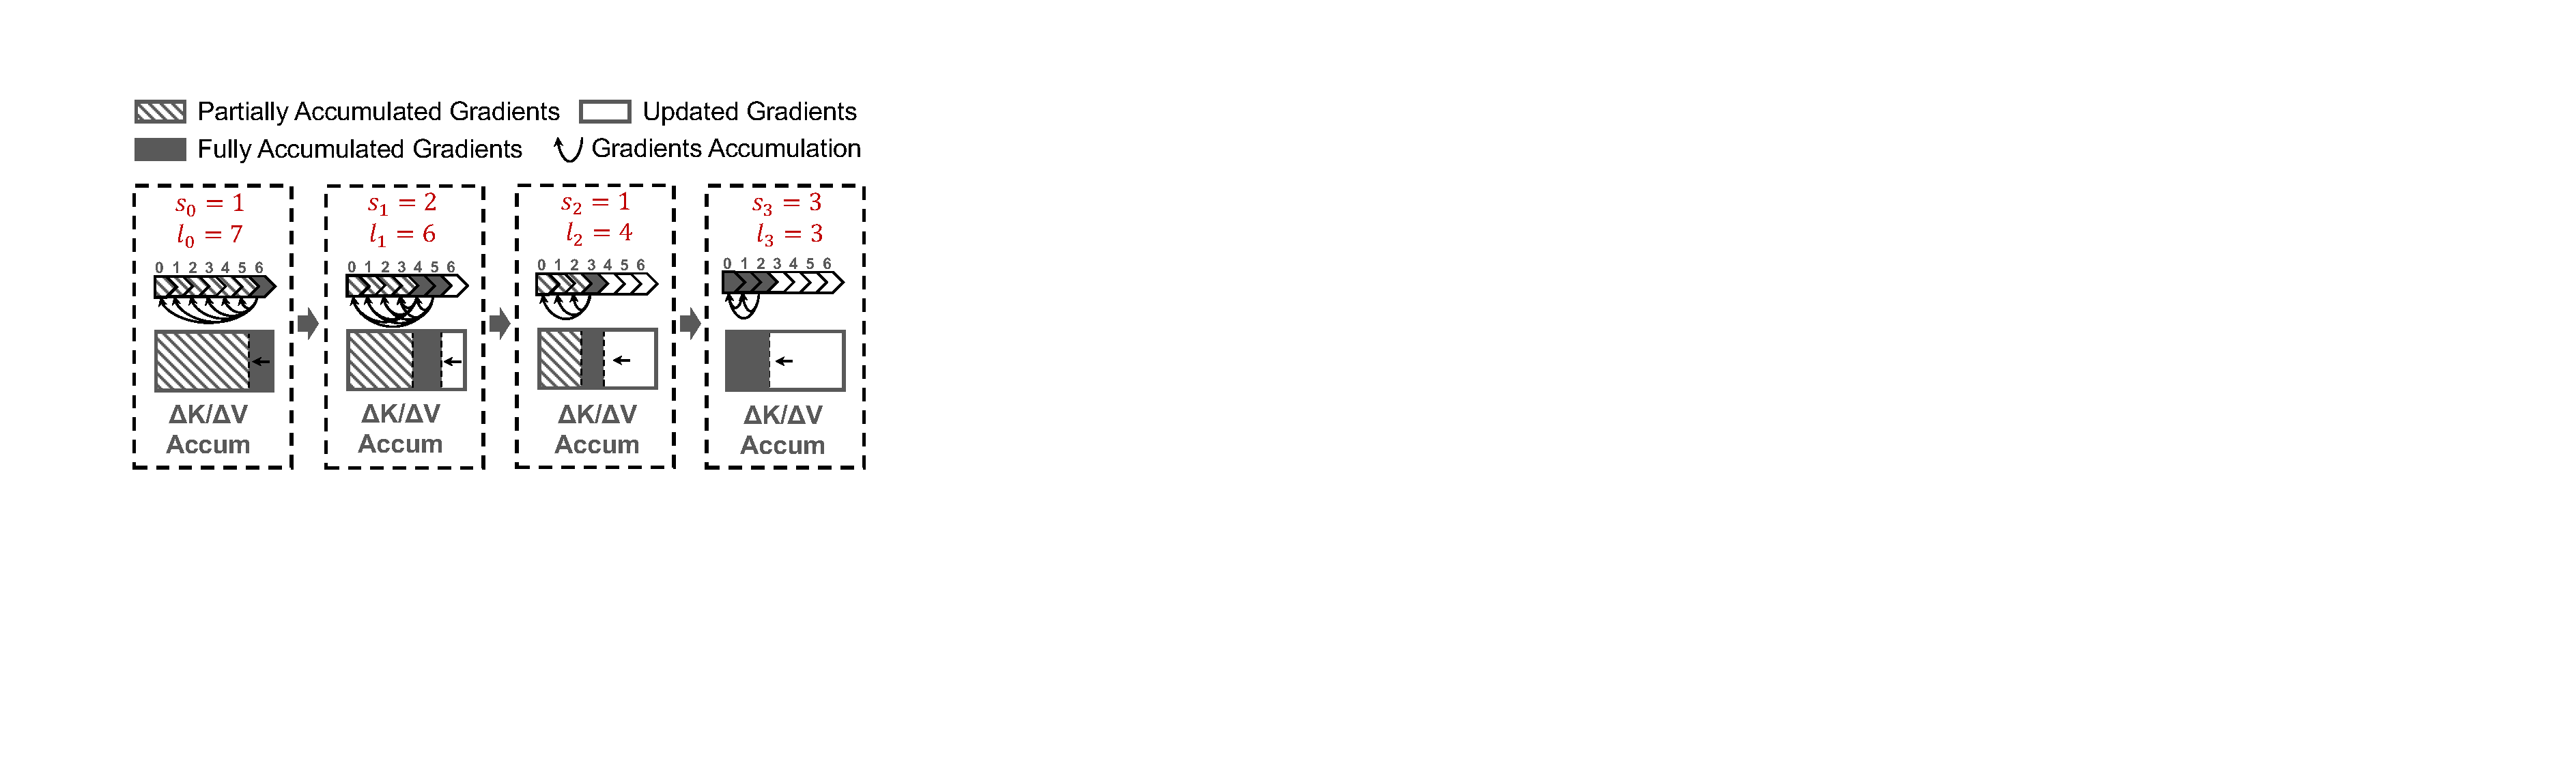
\includegraphics[width=0.8\linewidth]{figs/blockwise_back2.pdf}
    \caption{Illustration of KV gradients accumulation in the backward pass of \sys's token-level finetuning mechanism, where $s_j$ and $l_j$ are the window length and the starting position of the $j$-th slice of the sequence.}
    \label{fig:token-level-backword}
\end{figure}

\subsection{Token-Level Finetuning}
\label{subsec:incremental_finetuning}

Processing a finetuning request typically involves performing both forward and backward passes across all model layers for the entire input sequence.
When co-served with inference requests, this sequence-level execution can significantly interfere with the token-wise inference kernels and degrade system goodput---this is, the effective inference throughput that meets latency SLOs.

While sequence-level parallelism~\cite{megatron-sp, deepspeed-ulysses} could help reduce the added finetuning latency per GPU, this approach would suffer from coarse-grained scheduling, forcing the system to wait for entire finetuning sequences to complete before reallocating resources to handle inference bursts. 

To address this problem and maximize GPU utilization, \sys introduces a \textit{token-level finetuning} mechanism, detailed in \Cref{alg:token-level-finetuning}. The key idea is to decompose the finetuning computation into smaller steps using a dynamic sliding window over tokens. This window spans both the forward and backward passes, with its size dynamically determined by the hybrid token scheduler (line 4 and 15) to ensure that inference requests continue to meet their SLO constraints (\S\ref{subsec:scheduler}). 

During the forward pass (lines 3-11), the finetuning sequence is partitioned into windows of $s_i$ tokens (line 5), which are incrementally fed into the model. The model processes each token window layer by layer (lines 7-8), computes the generative loss for the window (line 10), and then advances to the next set of tokens (line 11).
To preserve the semantic of full sequence-level finetuning, \sys caches key and value tensors---similar to incremental decoding in inference~\cite{yu2022orca}---as well as query tensors, which are reused during backward attention computations. This caching follows the {\em causal mask} constraint inherent in LLMs.

During the backward pass (lines 12-21), \sys executes the model layers in reverse order (line 13).
Within each layer, the finetuning request is again divided into token windows (lines 14-16). 
However, unlike the relatively straightforward forward pass, token-level backward execution of the attention module is more complex due to auto-regressive token dependencies.

Figure~\ref{fig:token-level-finetuning} illustrates the forward and backward PCGs of the attention module. When computing gradients for $s_j$ tokens, the resulting gradients $\Delta Q$, $\Delta K$, $\Delta V$ have shapes $[s_j, h]$ for queries but $[l_j, h]$ for keys and values due to autoregressive attention dependencies. \sys accumulates KV gradients across steps, applying them only after complete backward traversal. This accumulation strategy minimally increases memory consumption due to layer-wise execution enabling workspace memory reuse.

\begin{algorithm}[t]
\caption{Token-level finetuning mechanism.}
\label{alg:token-level-finetuning}
\begin{algorithmic}[1]
\State {\bf Inputs}: PEFT model $M$ depth of $N$; Finetuning request $r$ with sequence length of $L$
\State {\bf Outputs}: PEFT model gradients $\Delta M$
% \State $i\gets 0, l_0 \gets 0$ \Comment{Forward pass}
\For{$i\gets 0, l_0 \gets 0$; $l_i<L$; $i\texttt{++}$} \Comment{Forward pass}
\State $s_i\gets \Call{HybridTokenScheduler}{l_i, L}$ 
\State $r_i \gets \Call{Slice}{r, l_i, s_i}$
\State $X_{0,i} \gets \Call{Tokenize}{r_i}$
\For{model layer index $n \in \Call{Range}{0, N}$}
\State $X_{n+1, i}, Q_{n, i}, K_{n, i}, V_{n, i} \gets \Call{Forward}{M_n, X_{n, i}}$
\State $QKVCache_n\gets \Call{Append}{Q_{n, i}, K_{n, i}, V_{n, i}}$
\EndFor
\State $Loss_{i} \gets \Call{GenerativeLoss}{X_{N, i}, r_i}$
\State $l_{i+1}\gets l_i + s_i$
% \State $l_{i+1}\gets l_i + s_i$, $i\gets i+1$
% \EndWhile
\EndFor
% \State $j\gets 0, l_0 \gets L$ \Comment{Backward pass}
% \While{$l_j>0$}
\State $Y_{N}\gets Loss$
\For{model layer index $n \in \Call{Range}{N-1, -1, -1}$}
\For{$j\gets 0, l_0 \gets L$; $l_j>0$; $j\texttt{++}$} \Comment{Backward pass}
\State $s_j\gets \Call{HybridTokenScheduler}{l_j, 0}$
\State $Y_{n+1, j} \gets \Call{Slice}{Y_{n+1}, l_j, s_j}$
% \State $Y_{j,n}, \Delta K_i, \Delta V_i \gets \Call{Backward}{M_n, Y_{j,n-1}, QKVCache, \Delta KVAccum}$
\State $Y_{n, j}, \Delta K_{n, j}, \Delta V_{n, j} \gets \textsc{Backward}(M_n, Y_{n+1, j},$
\Statex \hfill $QKVCache_n, \Delta KVAccum_n)$
\State $\Delta KVAccum_n\gets\Call{Add}{\Delta K_{n, j}, \Delta V_{n, j}}$
\State $G_{n, j}\gets \Call{Slice}{\Delta KVAccum_n, l_j, s_j}$
\State $\Delta M_{n} \gets \Delta M_{n}+\Call{CalculateGrads}{M_n, G_{n, j}}$
\EndFor
\State $l_{j+1}\gets l_j-s_j$
\EndFor
% \State $l_{j+1}\gets l_j-s_j, j\gets j+1$
% \EndWhile
% \Function{Build}{$\m{G}, \m{I}$}
% \EndFunction
\State {\bf return} $\Delta M$
\end{algorithmic}
\end{algorithm}


\begin{figure}[t]
    \centering
    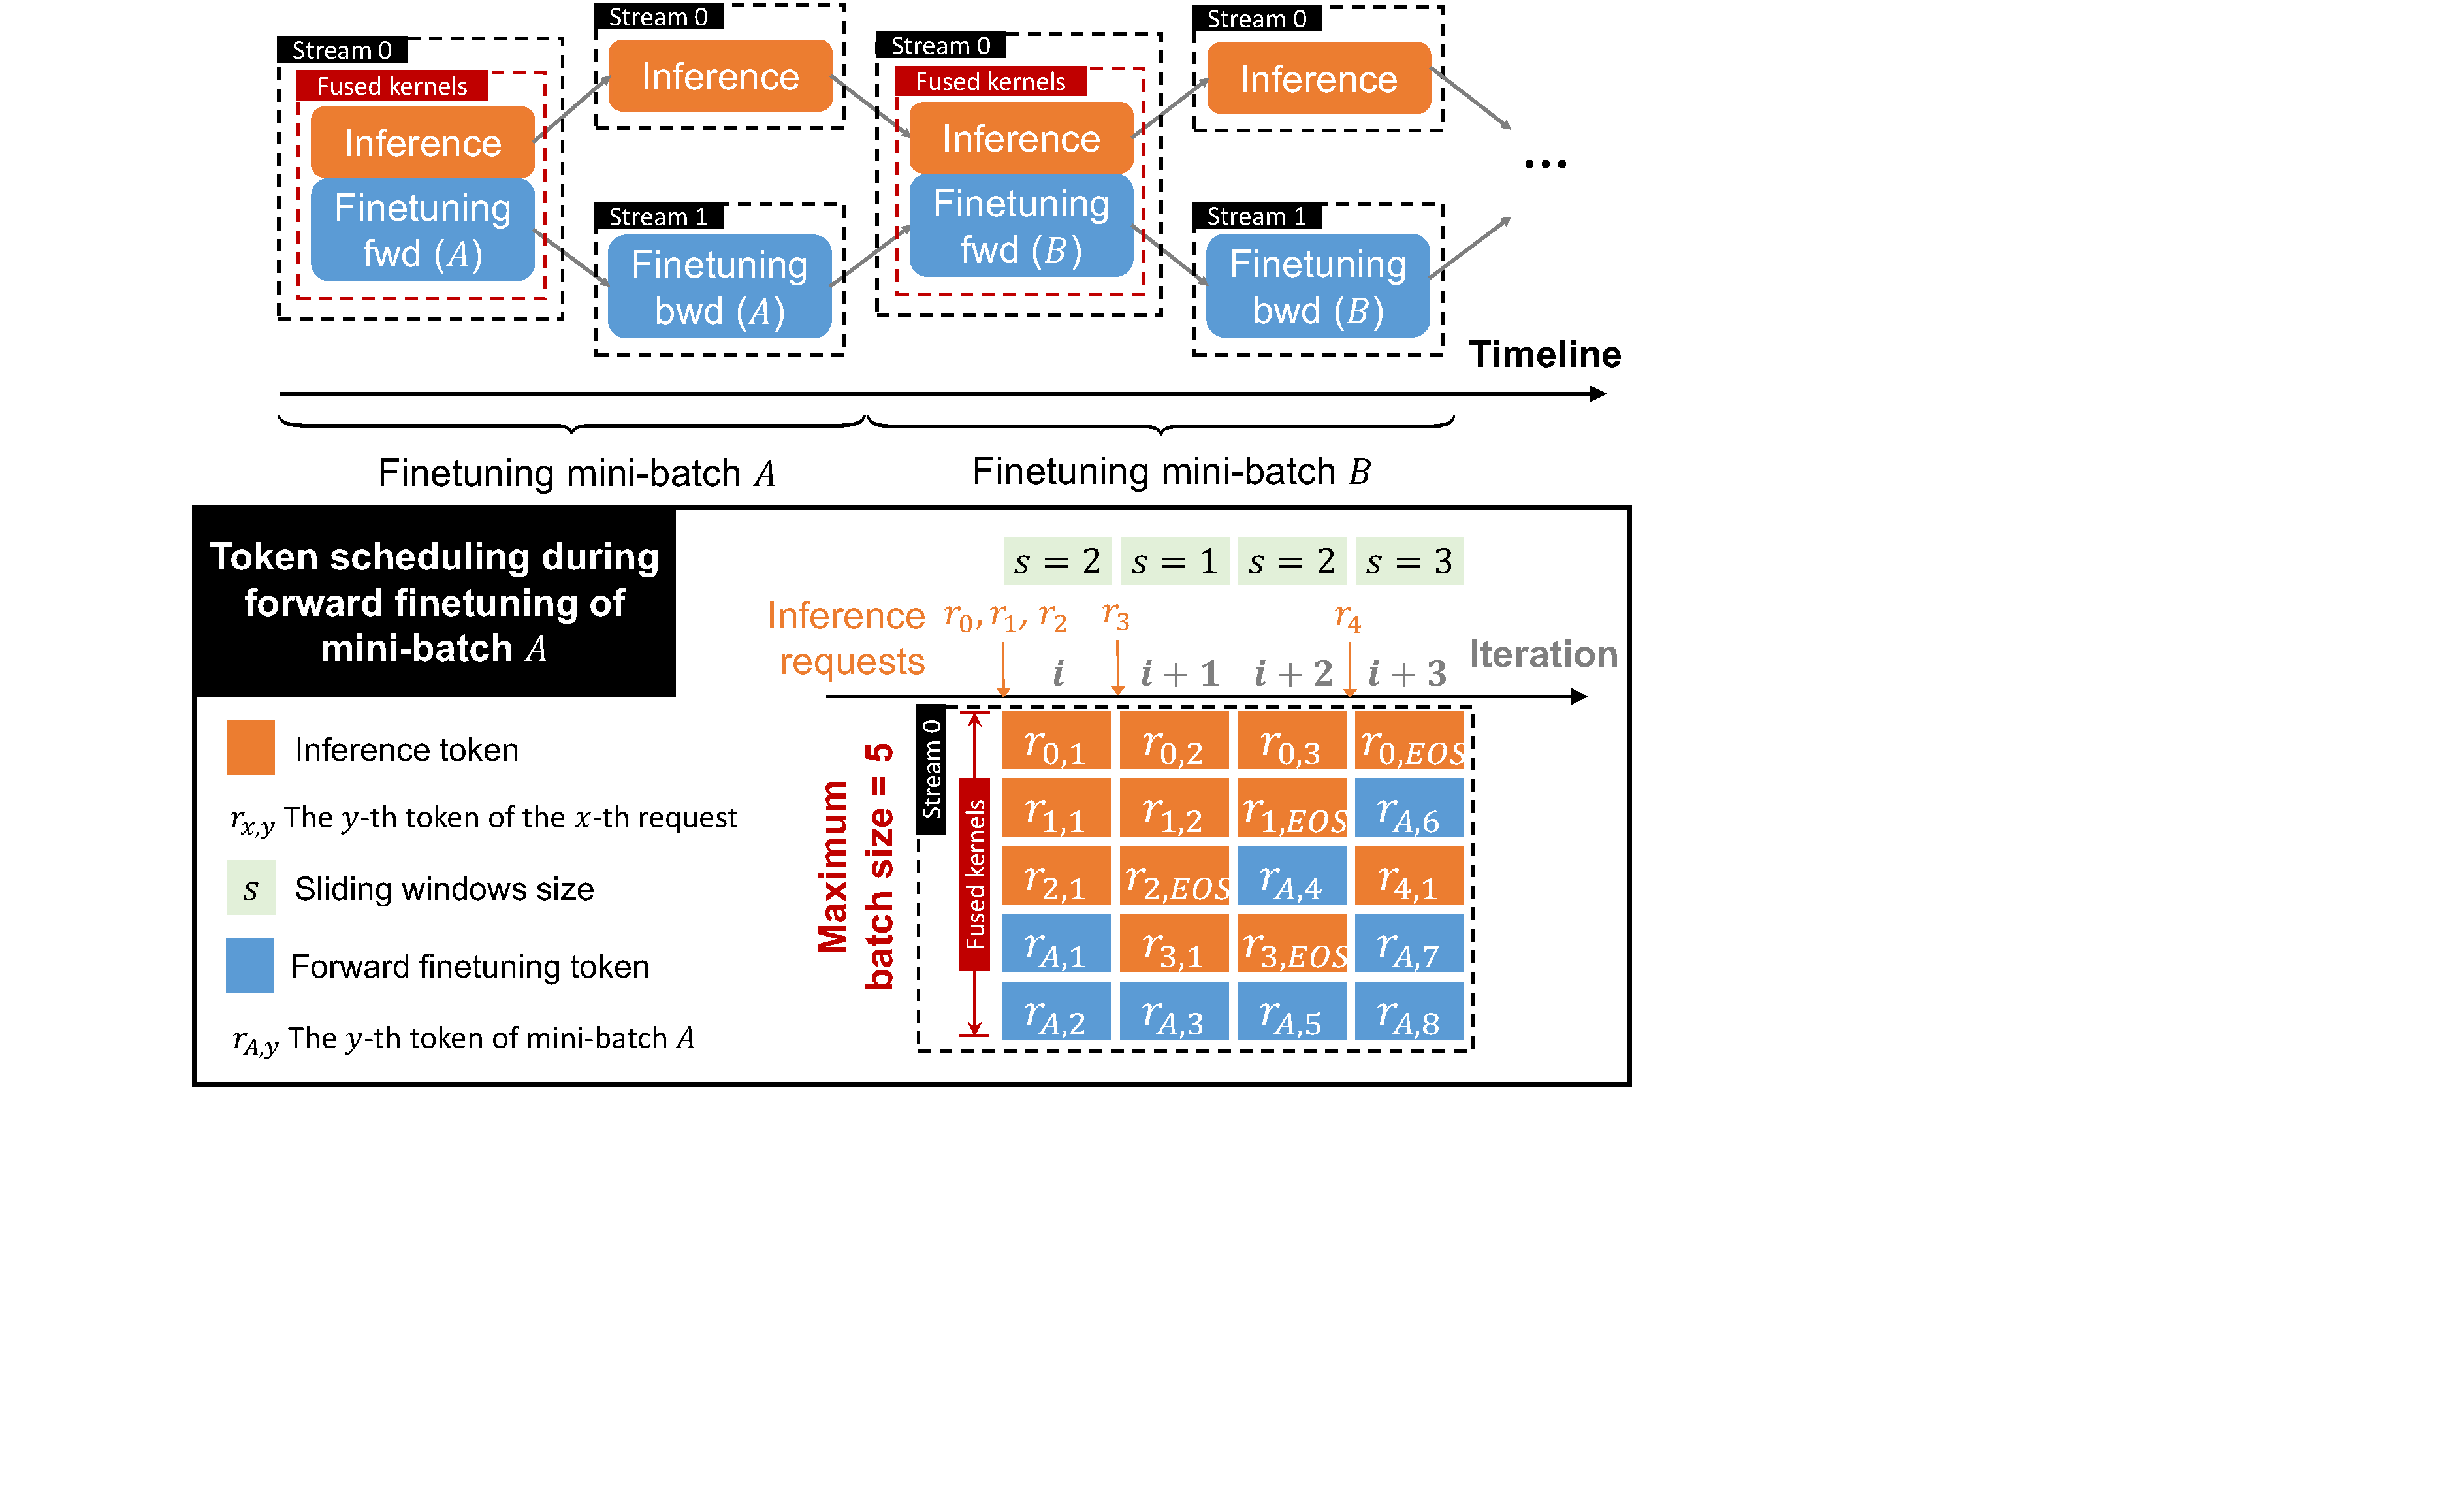
\includegraphics[width=\linewidth]{figs/token_level_scheduling4.pdf}
    \caption{Execution timeline and token scheduling when co-serving inference requests and a finetuning mini-batch.}
    % Numbers in parenthesis indicate the iteration numbers for serving and PEFT operators, respectively, and arrows show data dependencies between operators. 
    \label{fig:execution_timeline}
\end{figure}


\subsection{Hybrid Token Scheduler}
\label{subsec:scheduler}

\Sys's \textit{hybrid token scheduler} coordinates token-level GPU execution in two stages. 
%
First, \Sys determines the scheduling of available inference requests based on specific scheduling policies. By default, \sys adopts Orca's \textit{iteration-level scheduling}~\cite{yu2022orca}, which maintains a fixed maximum batch size and dynamically replaces each completed request with a new one whenever available.
%
To further mitigate blocking caused by long input sequences, \sys incorporates the chunked-prefill optimization~\cite{agrawal2024taming}.

Second, after determining the inference schedule for a given iteration, \sys opportunistically appends as many finetuning tokens as possible---determined by the sliding window size $s$---to maximize GPU utilization. The number of finetuning tokens added is determined automatically using the formula $s=\argmax f(c, s)\leq$SLO, where $f(\cdot, \cdot)$ is the latency estimation function and $c$ is the number of inference tokens scheduled in the current iteration. Here $f(\cdot, \cdot)$ is derived via offline profiling of the LLM's execution~\cite{narayanan2023cheaply}.
%
Such window-based, best-effort scheduling mechanism ensures that \sys can automatically adapt to inference workload fluctuations, maintaining inference SLOs while opportunistically allocating compute to finetuning tasks (\S\ref{sec:exp:dynamic}).

Figure~\ref{fig:execution_timeline} illustrates the execution timeline of \Sys and shows an example a token scheduling plan for a finetuning mini-batch $A$, under a representative inference requests arrival pattern (i.e., $r_0$ to $r_4$).
To preserve the semantics of finetuning, \sys enforces the execution dependencies between the forward and backward passes of each mini-batch.
During the forward pass, \sys leverages fused GPU kernels to jointly process both inference and finetuning tokens. This approach avoids additional kernel launch overhead and is enabled by the shared token-wise computation logic between inference and finetuning. In particular, finetuning tokens follow the same execution pattern and causal masking rules as inference tokens during the prefill phase, guaranteeing compatibility at the kernel level.
For the backward pass, \sys adapts a space-sharing approach, using two separate GPU streams: one for inference tokens and another for finetuning tokens. This design allows concurrent execution without interference.
